\newcommand{\signatuur}[2]{\ensuremath{%
  \vcenter{\offinterlineskip
    \halign{\hfil##\hfil\cr
            $\scriptstyle#1$\cr
            \noalign{\vskip1pt}
            $\scriptstyle#2$\cr}
  }}%
}

\chapter{Muzikale achtergrond}
\label{hoofdstuk:MA}

Aangezien deze thesis zal handelen over melodische transformaties wordt hieronder in het kort info gegeven over elementaire begrippen rond ritme en melodie van een muziekstuk en hoe deze voorgesteld kunnen worden. Voor lezers met een voorkennis in de muziekwereld zal dit onderdeel waarschijnlijk redundant zijn en kan er bijgevolg ook meteen overgegaan worden naar het volgende hoofdstuk. 

\section{Ritme}
In deze masterproef worden enkel melodische transformaties behandeld, waarbij het ritme ongewijzigd blijft. De tegenhangers hiervan zijn de ritmische transformaties\cite{thesis:thomas}, die in deze masterproef niet behandeld worden. Toch is het zeker nuttig om ook een zekere voorkennis te hebben van de betekenis van ritme in een muziekstuk. Melodie en ritme van een muziekstuk gaan namelijk hand in hand. Een basiskennis van ritmische begrippen zal dus zeker ook nuttig zijn voor het begrijpen van bepaalde melodische fenomenen.  

\subsection{Tijdssignaturen}
De tijdssignatuur geeft de ritmische structuur weer van het muziekstuk. Deze tijddssignatuur wordt weergegeven aan het begin van de notenbalk en ziet eruit als een breuk zonder streepje. Een voorbeeld hiervan is de vaak gebruikte \signatuur{3}{4} (of 'drie vierden'). In deze voorstelling staat het onderste getal voor welke nootlengte overeen komt met een tel. Het bovenste getal geeft weer hoeveel tellen in een maat voorkomen \cite{thesis:vincent}. In het voorbeeld van de signatuur \signatuur{3}{4} komt dit over met 4 tellen van lengte $\frac{1}{4}$. Voor de specifieke signatuur \signatuur{4}{4} (of 'vier vierden') heeft men nog een andere notatie, namelijk de letter C. Deze letter komt het woord \textit{common time}, aangezien deze signatuur zo typisch en veelvoorkomend is in moderne Westerse muziek. Figuur \ref{figuur:tijdssignatuur} geeft het gebruik van deze notatie weer. De figuur illustreert ook de 4 verschillende tellen van deze maatsoort.

\begin{figure}[!ht]
  \centering
  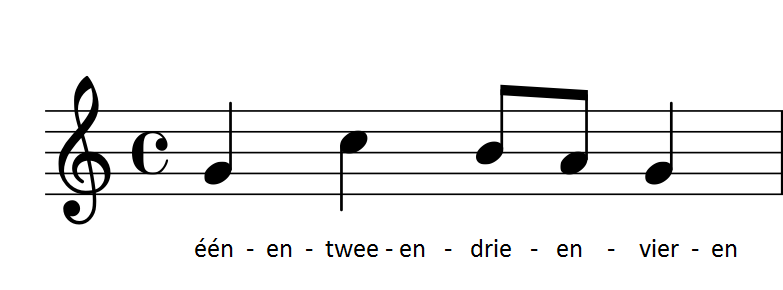
\includegraphics[width=0.5\textwidth]{1_Muzikale_Achtergrond/tijdssignatuur}
  \caption{Maat met voortekening van \textit{common time} tijdssignatuur.}
  \label{figuur:tijdssignatuur}
\end{figure}

\subsection{Tempo}
Een volgend belangrijk onderdeel dat het ritme van een muziekstuk bepaalt is het tempo. Het tempo van een stuk bepaalt namelijk de duur van de verschillende noten in het muziekstuk. Het temp wordt meestal uitgedrukt in aantal tellen per minuut. De lengte van een tel zelf wordt dan weer bepaald door de tijdssignatuur. Zo betekent bijvoorbeeld een tempo van 60 tellen voor een muziekstuk met signatuur \signatuur{3}{4} dat elke tel, ofwel elke kwartnoot, precies \'e\'en seconde duurt. 

\subsection{Nootlengtes}
De nootlengte is het laatste element dat de absolute duur van een noot zal bepalen. De nootlengte geeft de relatieve lengte van een noot weer ten opzichte van het tempo en de tijdssignatuur. De nootlengte wordt uitgedrukt door een breuk. Deze breuk heeft als relatieve lengte zijn verhouding tot de lengte van een tel. Zo zal een $\frac{1}{4}$-noot in \signatuur{3}{4} \'e\'en tel duren, en zal een $\frac{1}{8}$-noot in \signatuur{3}{4} twee tellen duren.

Een noot van hele lengte wordt aangeduid met een hol bolletje. Een noot van halve lengte wordt aangeduid met een half bolletje met een streep aan de rechterkant. Een $\frac{1}{4}$-noot wordt aangeduid zoals een halve noot maar dan met een vol bolletje. Een $\frac{1}{8}$-noot wordt voorgesteld door een vierde noot met een streepje vanboven. Vanaf een $\frac{1}{16}$-noot wordt er dan een streepje vanboven bijgezet telkens de nootlengte gehalveerd wordt. Deze notatie wordt ge\"illustreerd in figuur \ref{figuur:toonlengtes}. Door het gebruik van verbindingstekens(waarbij de nieuwe nootlengte de som is van de lengtes van de twee noten die verbonden zijn) kan men dan eender welke nootlengte bekomen die men maar wenst. 

\begin{figure}[!ht]
  \centering
  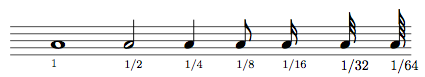
\includegraphics[width=0.5\textwidth]{1_Muzikale_Achtergrond/nootlengtes}
  \caption{Illustratie van een aantal veelvoorkomende nootlengtes.}
  \label{figuur:nootlengtes}
\end{figure}

\section{Melodie}
Naast ritme is het andere fundamentele bestanddeel van een muziekstuk de melodie. Waar het ritme de structuur van een muziekstuk weergeeft, is de melodie het voornaamste bestanddeel van de muziek dat een gevoel meegeeft aan het stuk. De melodie geeft een toonhoogte of frequentie mee aan elke noot. Aangezien deze thesis handelt over melodische transformaties is het van belang te weten wat het begrip ``melodie'' precies inhoudt. Het is namelijk dat gedeelte van een muziekstuk waarop een transformatie zal toegepast worden. Het ritme van een muziekstuk wordt in deze thesis onveranderd gelaten.

\subsection{Toonhoogte}
Toonhoogte kan in het algemeen op twee manieren voorgesteld worden. Een eerste manier is fysisch waarbij elke toon met een bepaalde frequentie overeenkomt, een andere manier is meer muziek-theoretisch, waarbij de toonhoogte als discreet beschouwd wordt. 

In deze masterproef zal met de laatste voorstellingswijze gewerkt worden. Dit omdat we noten willen transformeren naar nieuwe noten en niet frequenties naar nieuwe frequenties (die dan niet overeen komen met een noot en bijgevolg zeer waarschijnlijk niet goed gaan klinken in het geheel). Deze toonhoogte wordt dan voorgesteld door een naam. Er zijn twee naamgevingen die vaak gebruikt worden. Eerst is er de naamgeving waarbij de letters A t.e.m. G gebruikt worden. De andere naamgeving maakt gebruik van de woorden do -- re -- mi -- fa -- sol -- la -- si, de relatie tussen deze 2 naamgevingen wordt weergegeven in tabel \ref{tabel:toonhoogte}. Noten kunnen uiteraard ook op een notenbalk weergegeven worden, zie figuur \ref{figuur:toonladder} voor een visuele weergave. Hoe hoger de noot op de notenbalk, hoe hoger haar frequentie.

\begin{table}
  \centering
  \begin{tabular}{ c c c c c c c }
    A & B & C & D & E & F & G \\
    \hline
    \hline
    la & si & do & re & mi & fa & sol \\
  \end{tabular}
  \caption{Opsomming van de toonhoogtes in 2 verschillende benamingen.}
  \label{tabel:toonhoogte}
\end{table}

\begin{figure}[!ht]
  \centering
  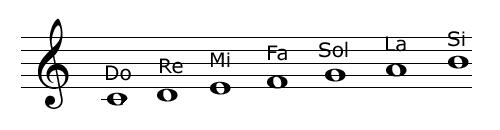
\includegraphics[width=0.5\textwidth]{1_Muzikale_Achtergrond/toonladder}
  \caption{Noten do t.e.m. si op een notenbalk.}
  \label{figuur:toonladder}
\end{figure}

\subsection{Octaaf en onderverdeling in toonhoogtes}
Een eenvoudige definitie van een octaaf is het interval tussen een gegeven toonhoogte en de toonhoogte met het dubbele van de frequentie van de eerste. Deze noten worden als zeer gelijkaardig ervaren en krijgen daarom dezelfde benaming (bijvoorbeeld beide een A). Hierdoor gaat men vaak in muzieknotatie wanneer men een bepaalde noot benoemt, ook aangeven tot welk octaaf de noot behoort (want een bepaalde noot komt met meerdere toonhoogtes overeen). Dit doet men door in subscript de index van het octaaf weer te geven, een A (of la) in het vierde octaaf wordt dan weergegeven door $A_{4}$.

Een octaaf wordt opgedeeld in 12 toonhoogtes. De afstand tussen elk paar van 2 opeenvolgende toonhoogtes wordt een halve toon genoemd. Hiervan zijn er slechts 7 tonen die ook deel uitmaken van de toonladder. De andere 5 noten worden voorgesteld op de notenbalk relatief ten opzichte van een van de nabijgelegen tonen die slechts een halve toon hier vanaf ligt door het gebruik van een kruis ($\sharp$) of een mol($\flat$). Een kruis dient om aan te duiden dat de noot die bedoeld wordt een halve toon hoger is dan de noot die ervoor staat. Een mol gebruikt men om aan te duiden dat de noot die bedoeld wordt een halve toon lager is dan de noot die net voor het molteken staat.

\subsection{Toonladders en toonaarden}
Zoals reeds vermeld werd in het vorige deel, bestaat een octaaf uit 12 tonen waarvan er slechts 7 tot de eigenlijke toonladder behoren. De noten binnen een toonladder worden bepaald door de intervallen tussen de noten. In het algemeen zijn er twee grote onderverdelingen om een toonladder te construeren. 

Een eerste resultaat wordt de ``grote toonladder'' genoemd. deze wordt bepaald door de opeenvolging van stappen 1-1-$\frac{1}{2}$-1-1-1-$\frac{1}{2}$. Het meeste elementaire voorbeeld van een toonladder die hieraan voldoet is de toonladder van ``Do-Groot'' waarbij volgende noten voldoen aan de opgegeven intervalafstanden: ``do - re - mi - fa - sol - la - si - do'', zoals weergegeven in figuur \ref{figuur:do_groot}. 

\begin{figure}[!ht]
  \centering
  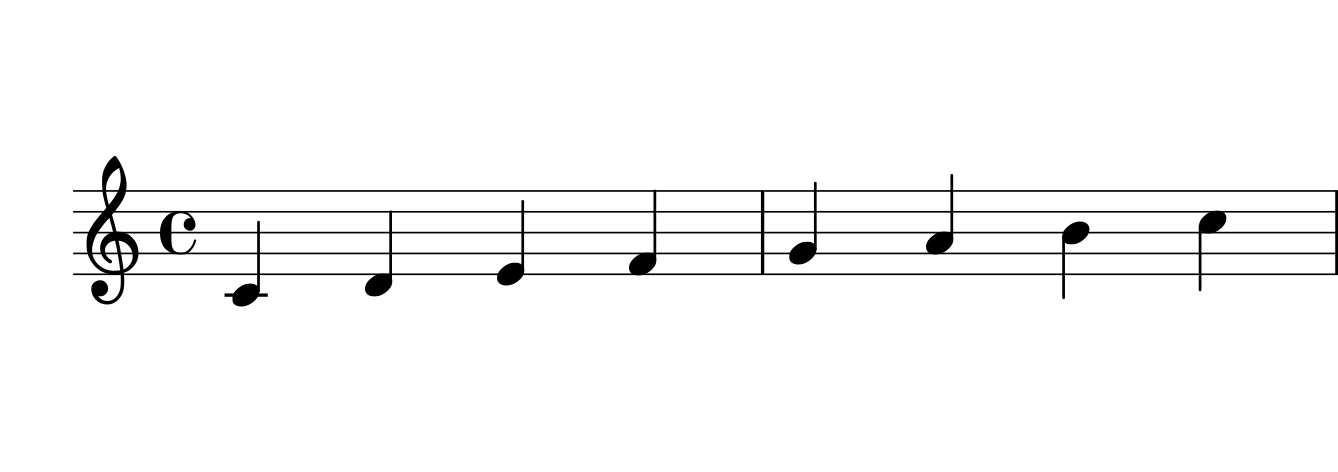
\includegraphics[width=0.5\textwidth]{1_Muzikale_Achtergrond/do_groot}
  \caption{Toonladder van ``Do Groot''}
  \label{figuur:do_groot}
\end{figure}

Een tweede mogelijkheid is de zogenaamde ``kleine toonladder''. In deze toonladder komen de intervalafstanden overeen met 1-$\frac{1}{2}$-1-1-$\frac{1}{2}$-1-1. Een concreet voorbeeld hiervan is de toonladder van ``La-Klein'' waarbij deze noten voldoen aan de voorwaarden: ``la - si - do - re - mi - fa - sol - la'', deze wordt weergegeven in figuur \ref{figuur:la_klein}. 

\begin{figure}[!ht]
  \centering
  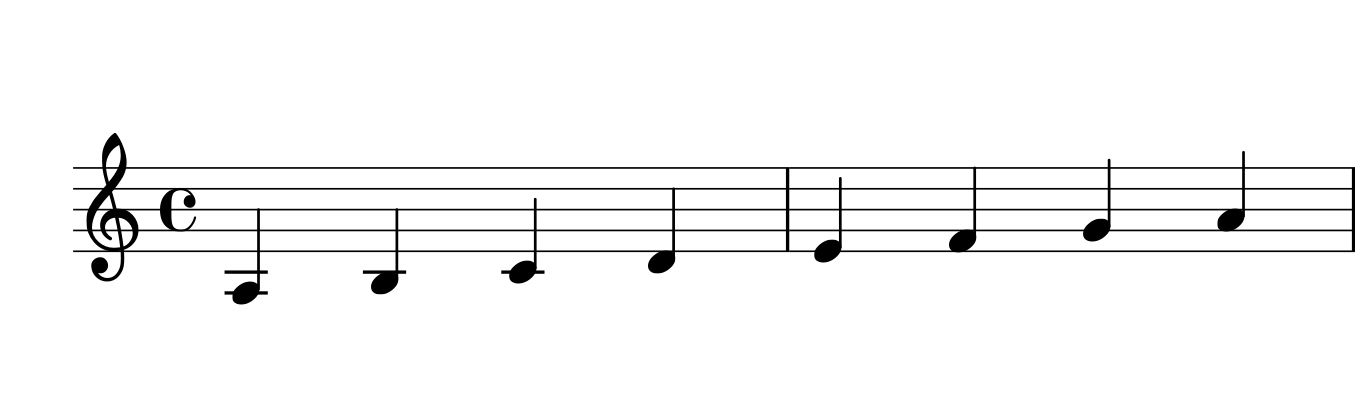
\includegraphics[width=0.5\textwidth]{1_Muzikale_Achtergrond/la_klein}
  \caption{Toonladder van ``La Klein''}
  \label{figuur:la_klein}
\end{figure}

Deze toonladder is de kleine versie van de toonladder van Do groot, aangezien ze dezelfde noten gebruikt, de toonladder is als het ware een verschuiving van die van Do groot. Het verschil tussen beide toonladders is dus de functie van elke noot in de bijhorende toonaarden. Iets wiskundiger verwoord is er ook een verschil van frequentie waarin bepaalde noten voorkomen in muziekstukken horende bij een kleine of grote toonladder \cite{book:musicAndProbability}. Van de kleine toonladders zijn ook nog een harmonische en melodische versie, die nog andere afstanden hanteren, maar aangezien deze niet zo vaak gebruikt worden, zou het te ver leiden deze ook te bespreken.

Het feit of een toonladder groot of klein is gaat vaak ook de sfeer bepalen van het muziekstukje. Zo zal een muziekstuk dat geschreven is in een grote toonladder eerder een vrolijk karakter hebben. Dit terwijl een stukje dat geschreven is in een kleine toonladder eerder een droeviger karakter zal hebben. 

Niet alleen de toonladder zelf, ook de noten in de toonladder hebben hun functie. Zo is bijvoorbeeld de eerste noot van een toonladder een rustpunt waarop het muziekstuk vaak be\"eindigd wordt. De vijfde noot wordt de dominant genoemd en is ook sterk vertegenwoordigd in het muziekstuk. Deze noot cre\"eert namelijk spanning. Vaak wordt deze spanning dan ook opgelost door een overgang naar de eerste noot, als rustpunt.


%%% Local Variables: 
%%% mode: latex
%%% TeX-master: "masterproef"
%%% End: 
